% ============================================================
%  AUTONOMOUS SOFTWARE AGENTS — FINAL PROJECT REPORT
%  Deliveroo.js: BDI + LLM Agent with PDDL Planning
% ============================================================
\documentclass[10pt,a4paper,twocolumn]{article}

\usepackage[utf8]{inputenc}
\usepackage[T1]{fontenc}
\usepackage[english]{babel}
\usepackage{geometry}
\usepackage{graphicx}
\usepackage{listings}
\usepackage{xcolor}
\usepackage{amsmath}
\usepackage{booktabs}
\usepackage{hyperref}
\usepackage{titlesec}
\usepackage{enumitem}
\usepackage{microtype}
\usepackage{caption}
\usepackage{float}
\usepackage{array}
\usepackage{tabularx}
\usepackage{tikz}
\usepackage{fancyhdr}
\usepackage{abstract}

\geometry{top=1.8cm, bottom=2.2cm, left=1.5cm, right=1.5cm, columnsep=0.55cm}

\hypersetup{colorlinks=true, linkcolor=blue!60!black, urlcolor=blue!60!black}

% --- Code listings style ---
\definecolor{bgcode}{rgb}{0.97,0.97,0.97}
\definecolor{frame}{rgb}{0.7,0.7,0.7}
\definecolor{kw}{rgb}{0.13,0.29,0.53}
\definecolor{cmt}{rgb}{0.25,0.50,0.35}
\definecolor{str}{rgb}{0.60,0.10,0.10}
\lstset{
  basicstyle=\footnotesize\ttfamily,
  backgroundcolor=\color{bgcode},
  frame=single,
  rulecolor=\color{frame},
  breaklines=true,
  breakatwhitespace=false,
  captionpos=b,
  numbers=none,
  xleftmargin=3pt,
  xrightmargin=3pt,
  aboveskip=4pt,
  belowskip=4pt,
  keywordstyle=\color{kw}\bfseries,
  commentstyle=\color{cmt}\itshape,
  stringstyle=\color{str}
}

% JavaScript language definition for the listings package
\lstdefinelanguage{JavaScript}{
  keywords={const,let,var,function,return,if,else,for,while,do,break,
            continue,async,await,class,new,this,true,false,null,undefined,
            throw,try,catch,of,in,static,import,export,from},
  morecomment=[l]{//},
  morecomment=[s]{/*}{*/},
  morestring=[b]{`},
  morestring=[b]{"},
  morestring=[b]{'},
  sensitive=true
}

% PDDL language definition
\lstdefinelanguage{PDDL}{
  keywords={define,domain,problem,requirements,types,predicates,action,
            parameters,precondition,effect,and,not,objects,init,goal,
            strips,typing},
  morecomment=[l]{;},
  sensitive=false
}

% --- Section spacing ---
\titlespacing{\section}{0pt}{8pt}{3pt}
\titlespacing{\subsection}{0pt}{5pt}{2pt}
\titlespacing{\subsubsection}{0pt}{4pt}{1pt}
\setlength{\parskip}{3pt}
\setlength{\parindent}{1em}

% --- Running header ---
\pagestyle{fancy}
\fancyhf{}
\fancyhead[L]{\small\textit{Deliveroo.js: BDI + LLM Agent with PDDL Planning}}
\fancyhead[R]{\small\thepage}
\renewcommand{\headrulewidth}{0.4pt}

% ============================================================
\title{%
  \vspace{-1.5em}%
  \textbf{Deliveroo.js: a BDI and LLM Solution\\
          with PDDL Planning for Autonomous Parcel Delivery}\\[4pt]
  \large Autonomous Software Agents — Final Project Report\\[2pt]
  \normalsize A.A.\ 2025--2026 \quad University of Trento
}
\author{Filippo Roseghini  ID: 267934. \texttt{roseghini.filippo@studenti.unitn.it}}
\date{}
% ============================================================

\begin{document}

% Title + abstract span both columns via \twocolumn trick
\twocolumn[
  \maketitle
  \begin{onecolabstract}
  This report presents the design and implementation of two autonomous agents
  for \textbf{Deliveroo.js}, a competitive multi-agent parcel delivery game.
  \textbf{Agent A} follows a Belief--Desire--Intention (BDI) architecture with
  utility-based option generation, A* pathfinding, and a three-level PDDL
  planning hierarchy covering tile navigation, task sequencing, and
  Sokoban-style crate recovery.  \textbf{Agent B} implements a
  Plan-and-Execute architecture backed by a large language model
  (Llama-3.3-70B via LiteLLM), enabling free-text mission interpretation
  with near-zero perceived latency through a hybrid startup mechanism.
  The two agents coordinate via a lightweight message-passing protocol
  over the game chat bus, supporting parcel handoff, relay mode, and
  team-wide constraint synchronisation.
  \end{onecolabstract}
  \noindent\textbf{Keywords:} BDI, PDDL, LLM, Multi-Agent Systems,
  Plan-and-Execute, Sokoban Planning, Deliveroo.js
  \vspace{1em}
  \hrule
  \vspace{0.5em}
  \tableofcontents
  \vspace{1em}
  \hrule
  \vspace{1.5em}
]

% ============================================================
\section{Introduction}
% ============================================================

This report documents the design and implementation of two autonomous software
agents for \textbf{Deliveroo.js}~\cite{deliveroojs}, a web-based multi-agent game in which agents
compete to maximise score by collecting and delivering parcels on a 2-D tile
grid.  Parcels decay in value over time, placing a premium on rapid
pick-up/delivery cycles and efficient path-planning.  The environment also
features directional tiles (conveyor belts), crates (Sokoban-style movable
obstacles), multiple delivery and spawn zones, and dynamic competition with
other agents.

We developed two agents with complementary architectures:
\begin{itemize}[noitemsep]
  \item \textbf{Agent A (BDI):} a classic Belief--Desire--Intention agent with
        A* pathfinding, real-time utility reasoning, and a PDDL recovery layer
        for Sokoban-style obstacle navigation (\texttt{agente3/}).
  \item \textbf{Agent B (LLM):} a Plan-and-Execute agent backed by a large
        language model (Llama-3.3-70B via LiteLLM~\cite{litellm}) capable of interpreting
        free-text mission objectives, issuing deterministic navigation actions,
        and replanning on failure (\texttt{agente\_llm/}).
\end{itemize}

Both agents share the same belief representation (\texttt{beliefs.js}) and
A* planner (\texttt{planner.js}) and coordinate through a lightweight
message-passing protocol (\texttt{[COORD]}) over the game's chat bus.

\begin{figure*}[!t]
\centering
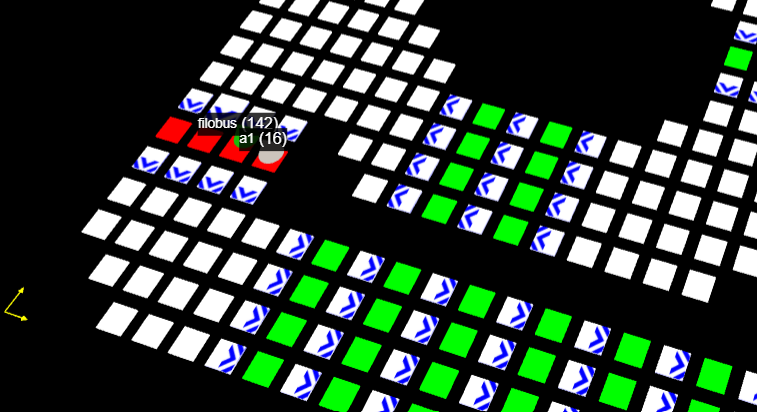
\includegraphics[width=0.72\linewidth]{setup.png}
\caption{Agent A (\textbf{filobus}, red, BDI, score 142) competing against a
         random agent (\textbf{a1}, white, score 16) on a map with directional
         conveyor tiles (blue arrows) and multiple delivery zones (green).
         The score gap illustrates the advantage of utility-driven option
         generation over random behaviour in the same environment.}
\end{figure*}

\begin{figure}[H]
\caption{System overview (render with \href{https://mermaid.live}{mermaid.live})}
\begin{lstlisting}[language={}]
flowchart LR
    Server["DeliverooJS Server"]
    subgraph AgentA ["Agent A — BDI (agente3/)"]
        direction TB
        BelA["beliefs.js\n(Beliefs)"]
        PlanA["planner.js\n(A*)"]
        AgA["agent.js\n(BDI loop)"]
        PDDL["pddlPlanner / pddlDelivery\n/ pddlCrates"]
    end
    subgraph AgentB ["Agent B — LLM (agente_llm/)"]
        direction TB
        BelB["beliefs.js\n(Beliefs)"]
        PlanB["planner.js\n(A*)"]
        AgB["agent_llm.js\n(Plan-and-Execute)"]
        LLM["LiteLLM\n(Llama-3.3-70B)"]
    end
    Server -- "onSensing / onMap /\nonConfig / onYou" --> AgentA
    Server -- "onSensing / onMap /\nonConfig / onYou" --> AgentB
    AgentA -- "emitMove / emitPickup\n/ emitPutdown" --> Server
    AgentB -- "emitMove / emitPickup\n/ emitPutdown" --> Server
    AgentA <-- "[COORD] messages\n(game chat)" --> AgentB
\end{lstlisting}
\end{figure}

% ============================================================
\section{Agent A: BDI Architecture}
\label{sec:bdi}
% ============================================================

Agent A is designed around the classic BDI model \cite{rao1995}, in which the
agent continuously cycles through belief revision, desire generation, and
intention selection.

\subsection{Environment Perception and Belief Revision}

Agent A maintains a continuously updated world model in \texttt{beliefs.js}
(\texttt{class Beliefs}).  Every \texttt{socket.onSensing} event triggers
\texttt{updateSensing(sensings, myPosition, sensingRadius)}, which applies the
following revision policy to the agent's belief state:

\begin{itemize}[noitemsep]
  \item \textbf{Parcel beliefs.} Parcels seen in the current sensing window
        are inserted or updated (position, reward, timestamp \texttt{lastSeen}).
        Parcels \emph{inside} the sensing radius but absent from \texttt{sensings}
        are removed (they have been picked up or expired).  Parcels \emph{outside}
        the radius are retained until a TTL derived from the server's decay rate
        expires, preventing premature deletion of high-value parcels momentarily
        out of view.
  \item \textbf{Agent beliefs.} Other agents observed in the sensing window are
        recorded by \texttt{id} with their last known position.  Stale entries
        older than 30\,s (\texttt{AGENT\_MEMORY\_MS}) are purged.
  \item \textbf{Crate beliefs.} Crate positions are tracked in a \texttt{Set}
        (\texttt{Beliefs.crates}).  Changes are only processed when a crate tile
        is inside the sensing radius, preserving the last known position of
        out-of-range crates as obstacles.
  \item \textbf{Map belief.} The static map is populated once from
        \texttt{socket.onMap} and never overwritten.  Delivery zones and spawn
        zones are extracted at load time into dedicated arrays.
  \item \textbf{Sensing radius calibration.} \texttt{sensingRadius} is
        initialised from \texttt{process.env.SENSING\_RADIUS} (fallback: 5) and
        updated dynamically via \texttt{socket.onConfig}, reading
        \texttt{config.GAME.player.observation\_distance}.  This ensures correct
        belief revision boundaries regardless of which server map is loaded.
\end{itemize}

\subsection{Desires: Option Generation and Utility Scoring}

\texttt{optionsGeneration()} is invoked on every sensing cycle and produces
exactly one \emph{predicate} (the intended next action).  Candidate actions are:
\texttt{go\_pick\_up}, \texttt{go\_deliver}, \texttt{patrol}, \texttt{crate\_nav},
and coordination predicates (\texttt{coord\_idle}, \texttt{coord\_goto\_wait},
\texttt{coord\_rendezvous}).

\subsubsection*{Pickup utility}
For each visible, non-blacklisted parcel $p$ the agent computes:
\[
  U_\text{pickup}(p) = \frac{\hat{R}(p, d_p)^2}{d_p}
\]
where $d_p$ is the Manhattan distance to $p$ and $\hat{R}(p, d_p)$ is the
estimated reward at arrival, accounting for the decay already accumulated since
the last sensing and the decay that will accrue during the $d_p$-step walk:
\[
  \hat{R}(p, d) = \max\!\bigl(0,\; r_p - (\Delta t_\text{elapsed} + d \cdot T_\text{step}) \cdot \lambda\bigr)
\]
with $\lambda$ the per-millisecond decay rate (from \texttt{Beliefs.getDecayRatePerMs})
and $T_\text{step}$ the per-move duration (auto-calibrated via EMA from actual
\texttt{emitMove} timings).  Parcels whose estimated arrival reward is $\leq 0$
are discarded entirely.

\subsubsection*{Delivery utility}
When the agent carries at least one parcel it evaluates each valid delivery zone
$z$ for:
\[
  U_\text{deliver}(z) = \frac{R_\text{carried}(t)}{d_z}
\]
where $R_\text{carried}(t)$ is the sum of currently carried rewards adjusted for
elapsed decay, and $d_z$ is the Manhattan distance to zone $z$.

\subsubsection*{Decision policy}
The agent delivers if (a) it is at capacity (\texttt{MAX\_CAPACITY} = 18 parcels),
(b) the batch size constraint from a team mission is satisfied, or (c)
$U_\text{deliver} > U_\text{pickup}$ and it already holds parcels.  Patrol is
chosen as a fallback when no parcel is visible and the agent has not recently
visited a spawn zone.

\subsubsection*{Blacklist and congestion map}
Unreachable parcels and delivery zones are temporarily banned
(\texttt{BAN\_DURATION\_MS} = 3 s, \texttt{blacklist.parcels / .zones}) to avoid
oscillation.  Tile-level move rejections are recorded in a \texttt{congestionMap}
(TTL = 5 s, penalty $= 100$) that is passed to the A* planner as an additive cost
term, steering the agent around dynamically occupied tiles without permanent map
changes.

\subsection{Intentions: IntentionRevisionReplace and Plan Library}

We implement the \textbf{IntentionRevisionReplace} pattern: on each
\texttt{myAgent.push(predicate)} call, if the new predicate is \emph{identical}
to the current one, execution continues uninterrupted (intention stability); if
it differs, the running plan is stopped and the new predicate is pursued
immediately (reactivity).  This single invariant avoids a dedicated watchdog
timer and makes the agent both stable under sustained pursuit of the same
objective and immediately responsive to better opportunities.

\begin{figure}[H]
\caption{Core of the \texttt{IntentionRevisionReplace} class (\texttt{agent.js})}
\begin{lstlisting}[language=JavaScript]
async push(predicate) {
    // Stability: identical predicate -> do not interrupt the running plan
    if (JSON.stringify(predicate) ===
        JSON.stringify(this.currentPredicate)) return;

    // Reactivity: new predicate -> stop current plan and start the new one
    if (this.currentPlan) this.currentPlan.stop();
    this.currentPredicate = predicate;

    // Scan the plan library for the first applicable plan
    for (const PlanClass of planLibrary) {
        if (PlanClass.isApplicableTo(predicate[0])) {
            this.currentPlan = new PlanClass();
            await this.currentPlan.execute(...predicate);
            return;
        }
    }
    throw new Error(`No plan for predicate: ${predicate[0]}`);
}
\end{lstlisting}
\end{figure}


\noindent The \textbf{Plan Library} contains the following plans, tried in order
until one succeeds:

\begin{center}
\footnotesize
\begin{tabularx}{\columnwidth}{@{} l l X @{}}
\toprule
\textbf{Plan} & \textbf{Trigger predicate} & \textbf{Behaviour} \\
\midrule
\texttt{GoPickUp}       & \texttt{go\_pick\_up x y id}    & A* to $(x,y)$, \texttt{emitPickup} \\
\texttt{GoDeliver}      & \texttt{go\_deliver x y}         & A* to $(x,y)$, \texttt{emitPutdown} \\
\texttt{Patrol}         & \texttt{patrol x y}              & A* to nearest unvisited spawn zone \\
\texttt{CrateNavigate}  & \texttt{crate\_nav x y}          & PDDL Sokoban solver (§\ref{sec:pddl}) \\
\texttt{CoordIdle}      & \texttt{coord\_idle}             & busy-wait (freeze command active) \\
\texttt{CoordGotoWait}  & \texttt{coord\_goto\_wait x y d} & A* to rendezvous tile, wait for release \\
\texttt{CoordRendezvous}& \texttt{coord\_rendezvous x y}   & A* to mid-point for handoff \\
\bottomrule
\end{tabularx}
\end{center}

\noindent Plans that fail (A* returns \texttt{null}, move rejected
\texttt{MAX\_MOVE\_FAILS} times consecutively) propagate the failure to
\texttt{IntentionRevisionReplace}, which allows the next \texttt{optionsGeneration}
cycle to choose a different goal.

\begin{figure}[H]
\caption{BDI control loop of Agent A}
\begin{lstlisting}[language={}]
flowchart TD
    S([socket.onSensing]) --> BR[Belief Revision\nupdateSensing]
    BR --> OG[optionsGeneration\ncompute U_pickup and U_deliver]
    OG --> |"coord mode active"| CM[Coordination predicate\ncoord_idle / goto_wait / rendezvous]
    OG --> |"hasParcels and U_deliver wins"| GD[go_deliver x y]
    OG --> |"U_pickup wins"| chG{reachableByAStar?}
    chG --> |yes| GP[go_pick_up x y id]
    chG --> |"no and mapHasCrates"| CN[crate_nav x y]
    OG --> |"no parcels visible"| PT[patrol x y]
    GP & GD & PT & CN & CM --> IR[IntentionRevisionReplace\nstop if predicate changed]
    IR --> PL[Plan Library lookup]
    PL --> EX[Plan.execute\nA* path or PDDL sequence]
    EX --> |"emitMove / pickup / putdown"| S
    EX --> |"plan failed"| BL[blacklist target\nback to OG]
\end{lstlisting}
\end{figure}

\subsection{A* Pathfinder}

The A* implementation in \texttt{planner.js} models the grid as a
4-connected graph.  The heuristic is Manhattan distance ($h\text{-consistent}$,
$h(n) = |x_n - x_g| + |y_n - y_g|$).  Edge traversal respects two constraints
added over the baseline:
\begin{enumerate}[noitemsep]
  \item \textbf{Directional tiles.}  The tile type encodes the allowed
        direction (e.g.\ \texttt{'→'} blocks entry from the right).  The planner
        checks \texttt{tile.type} directly, fixing a bug in the original scaffold
        where the non-existent property \texttt{tile.direction} made the check
        always false.
  \item \textbf{Crates as absolute walls.}  Crate positions are passed as a
        \texttt{Set<string>} (\texttt{crateKeys}) and treated as impassable,
        because Agent A's A* does not model push sequences.  Multi-push
        traversal is delegated to the PDDL Sokoban planner (§\ref{sec:pddl}).
\end{enumerate}

\noindent Before accepting any push that would move a crate, the planner verifies
\textbf{connectivity invariants} via a multi-source BFS from delivery zones:
all spawn zones and the agent's current position must remain reachable after the
push (\texttt{criticalZones} parameter).  This prevents the agent from
irreversibly walling itself off from spawn areas.

% ============================================================
\section{Agent B: LLM Agent and Multi-Agent Coordination}
\label{sec:llm}
% ============================================================

\subsection{Architecture: Plan-and-Execute}

Agent B follows the \textbf{Plan-and-Execute} schema~\cite{yao2023}: the LLM
is invoked \emph{only} to produce a high-level plan (sequence of tool calls),
while all low-level execution (navigation, pickup, delivery) is handled by
deterministic code with zero additional LLM calls.

\subsubsection*{Hybrid startup}
Because LLM inference takes 3--8 s, the agent \emph{does not block} at startup.
It immediately executes a deterministic fallback plan (top-$k$ parcels by
utility, greedy delivery) while \texttt{llmPlan()} runs in the background.  As
soon as the LLM response arrives, the agent adopts it, discarding the fallback
mid-flight if necessary.  This yields perceived zero latency for the observer
while satisfying the requirement that the LLM always drives planning.

\subsubsection*{LLM-Memory}
Before each plan request, \texttt{buildLLMMemory()} assembles a structured
context block:
\begin{itemize}[noitemsep]
  \item \textbf{Objective:} the current mission text (natural language or
        autonomous).
  \item \textbf{Environment observation} (\texttt{get\_visible\_environment()}):
        agent position, score, parcels sorted by utility with estimated arrival
        reward, delivery zone distances, active mission constraints.
  \item \textbf{Agent memory:} last 8 action outcomes (objective $\to$ result),
        kept in a rolling buffer (\texttt{agentMemory}).  Enables the LLM to
        avoid repeating recently failed actions.
  \item \textbf{BDI partner status:} last coordination message from Agent A.
\end{itemize}

\subsubsection*{Tool catalogue}
The LLM receives the following deterministic tools:
\texttt{navigate\_to}, \texttt{pick\_up}, \texttt{put\_down},
\texttt{drop\_here}, \texttt{calculate}, \texttt{reply\_to\_sender},
\texttt{send\_message\_to\_partner},
\texttt{avoid\_tiles}, \texttt{set\_delivery\_batch},
\texttt{set\_delivery\_bonus}, \texttt{set\_zero\_value\_tiles},
\texttt{set\_max\_parcel\_reward}, \texttt{clear\_mission\_rules},
\texttt{rendezvous}, \texttt{handoff\_to\_partner}.

\subsubsection*{Opportunistic pickup}
\texttt{navigate\_to} picks up any parcel on each traversed tile at zero extra
LLM cost.  This is suppressed when a \texttt{deliverBatchSize} constraint is
active (to avoid accidentally over-filling the stack) or when a
\texttt{maxParcelReward} constraint would be violated.

\subsubsection*{Replanning}
If an executed tool returns a failure string (e.g.\ \emph{"no path to x,y"},
\emph{"parcel expired"}), the agent invokes \texttt{llmPlan(memory, replanNote)}
with the failure note appended to the context.  Replanning is capped at
\textbf{3 attempts per objective} to bound LLM costs; a fourth failure aborts
the objective and logs it to \texttt{agentMemory}.

\begin{figure}[H]
\caption{Plan-and-Execute loop of Agent B}
\begin{lstlisting}[language={}]
flowchart TD
    OBJ([New objective\n natural language or autonomous]) --> HYB
    HYB[Hybrid startup\nrun deterministic fallback\nllmPlan in background] --> MEM
    MEM[buildLLMMemory\nobservation + history + mission rules] --> LLP
    LLP[llmPlan\n1 LLM call -> PLAN a1..aN] --> ADOPT
    ADOPT[Adopt LLM plan\ndiscard fallback if running] --> EXEC
    EXEC[Executor\niterate a1..aN, 0 LLM calls] --> |"tool result OK"| NEXT
    NEXT{More actions?} --> |yes| EXEC
    NEXT --> |no| DONE([Objective complete\nlog to agentMemory])
    EXEC --> |"tool failed"| REPL{replan count\n< 3?}
    REPL --> |yes| MEM
    REPL --> |no| DONE
\end{lstlisting}
\end{figure}

\subsection{Challenge 2: Atomic Missions (Level 1)}

Atomic missions arrive as natural-language text from an external agent via
\texttt{socket.on('msg')}.  Agent B interprets the objective through the LLM and
executes the appropriate tool sequence.  Notable implementation choices:

\begin{itemize}[noitemsep]
  \item \textbf{Arithmetic evaluation.}  Coordinates expressed as expressions
        (e.g.\ \texttt{"move to x=4*2 y=(1+3)*3"}) are evaluated by a safe
        recursive-descent parser (\texttt{safeEvalArithmetic}), which accepts
        only digits and the four arithmetic operators — no \texttt{eval()} is
        ever called.
  \item \textbf{Directed replies.}  \texttt{reply\_to\_sender(msg)} uses
        \texttt{socket.emitSay(activeSenderId, msg)} rather than
        \texttt{emitShout}, routing the answer to the requesting agent with
        $O(1)$ overhead regardless of spatial proximity.
  \item \textbf{Extreme tile queries.}  \texttt{getMapExtremes()} pre-computes
        the leftmost, rightmost, topmost, and bottommost walkable tiles once at
        map load time; the result is injected into the LLM context so the model
        can resolve missions such as \emph{"drop a package in the leftmost tile"}
        without guessing grid coordinates.
\end{itemize}

\noindent The following trace illustrates a typical Level 1 interaction.
The LLM receives the mission as plain text; its JSON response is parsed by
\texttt{llmPlan()} and handed directly to the executor without further model calls.

\begin{figure}[H]
\caption{Illustrative LLM interaction for a Level 1 atomic mission}
\begin{lstlisting}[language={}]
=== MISSION ===
"Drop a package in the leftmost tile."

=== LLM RESPONSE (parsed JSON) ===
{
  "thought": "I need to find the leftmost walkable tile. From the map
              extremes injected in context: leftmost = (-4, 2).
              I will navigate there and put down one parcel.",
  "plan": [
    { "tool": "navigate_to", "x": -4, "y": 2 },
    { "tool": "put_down" }
  ]
}

=== EXECUTOR TRACE ===
[LLM-EXEC] navigate_to -4 2  -> OK (arrived, opportunistic pickup: 0)
[LLM-EXEC] put_down          -> OK (1 parcel delivered, score +18)
[LLM-EXEC] plan complete, logging to agentMemory
\end{lstlisting}
\end{figure}

\subsection{Challenge 2: Persistent Strategy Constraints (Level 2)}

Level 2 missions impose \emph{persistent} behavioural constraints:
forbidden traversal tiles, exact delivery batch size, preferred or
zero-value delivery zones, and maximum parcel reward.  These are stored in
\texttt{missionConstraints} and \emph{enforced mechanically} in the execution
layer, not merely described in the LLM prompt:

\begin{itemize}[noitemsep]
  \item \texttt{avoid\_tiles} injects a penalty of 100\,000 into the A*
        congestion map for the forbidden tile, effectively routing around it
        without making it completely impassable.
  \item \texttt{set\_delivery\_batch(N)} blocks \texttt{put\_down} and
        disables opportunistic pickup until exactly $N$ parcels are carried.
  \item \texttt{set\_delivery\_bonus} / \texttt{set\_zero\_value\_tiles} bias
        \texttt{bestDeliveryZone()} to prefer or exclude specific tiles.
\end{itemize}

On every constraint change, \texttt{broadcastTeamRules()} serialises a complete
\texttt{[COORD] rules} snapshot to Agent A, keeping both agents' constraints
synchronised without differential updates.

\subsection{Multi-Agent Coordination (Level 3)}

\subsubsection*{[COORD] protocol}
Agents communicate over the game chat bus using a fixed-prefix protocol
(\texttt{[COORD]}) to avoid interference with mission messages.  Agent B
(LLM) acts as the \textbf{orchestrator}: it reads mission objectives in natural
language and issues directives to Agent A (BDI), which never parses free text.
The full command set is:

\begin{center}
\footnotesize
\begin{tabularx}{\columnwidth}{@{} l X @{}}
\toprule
\textbf{Command} & \textbf{Semantics} \\
\midrule
\texttt{[COORD] pos x y}          & position broadcast (both agents, periodic) \\
\texttt{[COORD] goto\_wait x y d} & BDI: move to nearest odd-row tile and wait \\
\texttt{[COORD] freeze}           & BDI: halt until released \\
\texttt{[COORD] release}          & both agents: resume normal play \\
\texttt{[COORD] rules k=v \ldots} & team-wide constraint snapshot (idempotent) \\
\texttt{[COORD] fetch id x y}     & BDI: pick up parcel \textit{id} at $(x,y)$ (handoff) \\
\texttt{[COORD] arrived}          & sender has reached the rendezvous point \\
\bottomrule
\end{tabularx}
\end{center}

\subsubsection*{Closest-commits parcel allocation}
Both agents independently apply the \textbf{closest-commits} heuristic (slide 9):
parcel $p$ is allocated to the agent with the lower Manhattan distance to it;
ties are broken by agent ID (lower ID wins).  No central allocator is needed;
each agent locally decides whether to pursue or ignore $p$.

\subsubsection*{Handoff and relay mode}
For missions requiring inter-agent parcel transfer, Agent B executes
\texttt{handoff\_to\_partner()}: it drops carried parcels at a midpoint tile,
sends a \texttt{[COORD] fetch id x y} for each dropped parcel, and activates
\texttt{relayMode}.  In relay mode, Agent B collects parcels but never delivers
them, instead continually dropping them for Agent A; Agent A ignores all
non-fetch objectives and focuses solely on pickup and delivery.

\begin{figure}[H]
\caption{Coordination sequence for a handoff mission}
\begin{lstlisting}[language={}]
sequenceDiagram
    participant LLM as Agent B (LLM)
    participant BDI as Agent A (BDI)
    participant SRV as DeliverooJS Server

    Note over LLM: receives NL mission via socket.msg
    LLM->>LLM: llmPlan -> [handoff_to_partner]
    LLM->>BDI: [COORD] rules relay=1
    Note over BDI: enters Clean Relay Mode
    LLM->>SRV: emitMove (navigate to midpoint)
    LLM->>SRV: emitPutdown (drop parcels)
    LLM->>BDI: [COORD] fetch p1 x y
    LLM->>BDI: [COORD] fetch p2 x y
    BDI->>SRV: emitMove (navigate to parcel)
    BDI->>SRV: emitPickup
    BDI->>SRV: emitMove (navigate to delivery zone)
    BDI->>SRV: emitPutdown
    loop periodic
        BDI->>LLM: [COORD] pos bx by
        LLM->>BDI: [COORD] pos lx ly
    end
    Note over LLM: next cycle: pick more parcels for relay
\end{lstlisting}
\end{figure}

% ============================================================
\section{PDDL Planning}
\label{sec:pddl}
% ============================================================

We integrate PDDL~\cite{mcdermott1998} planning at \textbf{three distinct levels}
of abstraction, each addressing a different planning sub-problem.  All three
modules call the \texttt{@unitn-asa/pddl-client} library (\texttt{onlineSolver})
to submit a domain+problem pair to the \texttt{solver.planning.domains}
service~\cite{planningdomains}.

\subsection{Navigation Planner (\texttt{pddlPlanner.js}) — tile-level STRIPS}

When the environment variable \texttt{USE\_PDDL\_PLANNER=true}, Agent A
replaces its A* planner with an external PDDL solver.  The domain models
each walkable tile as an object and encodes movement constraints (including
directional arrows) as binary predicates
\texttt{(right/left/up/down ?from ?to)}.  This is a pure STRIPS problem with
$O(|T|^2)$ facts in the worst case, kept tractable by a bounding-box scoping
strategy (at most \texttt{MAX\_PDDL\_TILES} = 600 tiles).

If the solver fails or times out, execution transparently falls back to the A*
planner (no interruption of gameplay).  This planner is primarily used to
demonstrate PDDL integration; the default runtime uses A* for performance.

\subsection{Task-Level Delivery Planner (\texttt{pddlDelivery.js}) — POI graph}

Activated by \texttt{USE\_PDDL\_DELIVERY=true}, this planner operates at the
\textbf{means-end reasoning} level of the BDI architecture.  Instead of tiling
the whole grid, it abstracts the world as a \emph{graph of Points of Interest}:
the agent's current position, up to \texttt{maxParcels} = 8 high-utility parcel
locations, and up to \texttt{maxZones} = 4 nearest delivery zones.  Real-world
travel costs between POIs are pre-computed by the A* planner.

\subsubsection*{Domain}
\begin{itemize}[noitemsep]
  \item \textbf{Predicates:} \texttt{(at ?loc)}, \texttt{(parcel-at ?p ?loc)},
        \texttt{(carrying ?p)}, \texttt{(delivered ?p)}.
  \item \textbf{Actions:} \texttt{goto ?from ?to} (moves the agent between
        reachable POI pairs), \texttt{pick-up ?p ?loc} (precondition: at ?loc,
        parcel-at ?p ?loc), \texttt{put-down ?p ?dz} (precondition: carrying ?p,
        at ?dz, delivery zone).
\end{itemize}

\subsubsection*{Problem}
The problem encodes the agent's current position as the initial \texttt{(at
agent-pos)}, lists all parcel facts, and sets the goal to
$\bigwedge_{p \in P} \texttt{(delivered } p\texttt{)}$.  The PDDL solver
returns an optimal task-level sequence (optimal w.r.t.\ number of actions, not
travel distance — a known limitation of STRIPS without \texttt{:action-costs}).
A 30 s cooldown (\texttt{PDDL\_FAIL\_COOLDOWN\_MS}) prevents hammering the
solver after a network failure.

\subsection{Sokoban Crate Planner (\texttt{pddlCrates.js}) — push-sequence recovery}

This is the highest-complexity PDDL component.  It is invoked by the
\texttt{CrateNavigate} plan when A* returns \texttt{null} on a map that contains
crates (\texttt{mapHasCrates = true}).  It computes the full multi-push sequence
needed to clear a path to the goal tile.

\subsubsection*{Activation guard}
The planner is never invoked on crate-free maps.  On such maps, an A* failure
means a genuine wall; calling the Sokoban solver would be both incorrect and
wasteful.  The \texttt{mapHasCrates} flag is set once in
\texttt{socket.onMap} after \texttt{Beliefs.updateMap} reports
\texttt{crates.size > 0}.

\subsubsection*{Domain}
\begin{itemize}[noitemsep]
  \item \textbf{Predicates:} \texttt{(at ?t)}, \texttt{(right/left/up/down ?a ?b)}
        (filtered for directional tiles — used for agent movement),
        \texttt{(adj-right/left/up/down ?a ?b)} (raw adjacency — used for crate
        push destination, as the server does not apply conveyor constraints to the
        \emph{destination} of a pushed crate), \texttt{(crate-at ?c ?t)},
        \texttt{(yellow ?t)} (tile that can receive a pushed crate),
        \texttt{(crate-free ?t)} (asserted for every walkable tile not occupied by
        a crate; mandatory under the STRIPS closed-world assumption).
  \item \textbf{Actions:} \texttt{move-right/left/up/down} (precondition:
        \texttt{crate-free} on target tile) and \texttt{push-right/left/up/down}
        (precondition: crate on target tile, yellow and free destination).
\end{itemize}

\noindent The key design decision in this domain is the dual-adjacency scheme:
agent movement uses \texttt{right/left/up/down} (conveyor-aware filtered
predicates), while crate destinations use \texttt{adj-right/left/up/down}
(raw adjacency), because the server does not apply conveyor constraints to
the landing tile of a pushed crate.

\begin{figure}[H]
\caption{PDDL \texttt{push-right} action from \texttt{pddlCrates.js}}
\begin{lstlisting}[language=PDDL]
; Agent at ?a pushes the crate at ?t1 one step right into ?t2.
; Requires: agent can move right to the crate (?a -right-> ?t1),
;           and the crate's landing tile (?t2) is yellow and free.
(:action push-right
 :parameters (?a ?t1 ?t2)
 :precondition (and (at ?a)
                    (right ?a ?t1)       ; conveyor-aware: agent can step right
                    (crate-at ?t1)       ; a crate occupies the target tile
                    (adj-right ?t1 ?t2)  ; raw adjacency for the landing tile
                    (yellow ?t2)         ; only yellow tiles accept crates
                    (crate-free ?t2))    ; landing tile must be unoccupied
 :effect (and (not (at ?a))   (at ?t1)
              (not (crate-at ?t1)) (crate-at ?t2)
              (crate-free ?t1)    (not (crate-free ?t2))))
\end{lstlisting}
\end{figure}

\subsubsection*{Scoping}
The full map is included if it has $\leq 150$ walkable tiles
(\texttt{MAX\_PDDL\_CRATE\_TILES}).  For larger maps a bounding box between
start and goal is expanded by a margin of 4--8 tiles in each direction
(proportional to the start-to-goal distance), ensuring that crates just outside
the naive box are not treated as invisible walls.  If the scoped problem exceeds
the tile or crate budget, the planner returns \texttt{null} and the agent falls
back to blacklisting.

\begin{figure*}[!t]
\centering
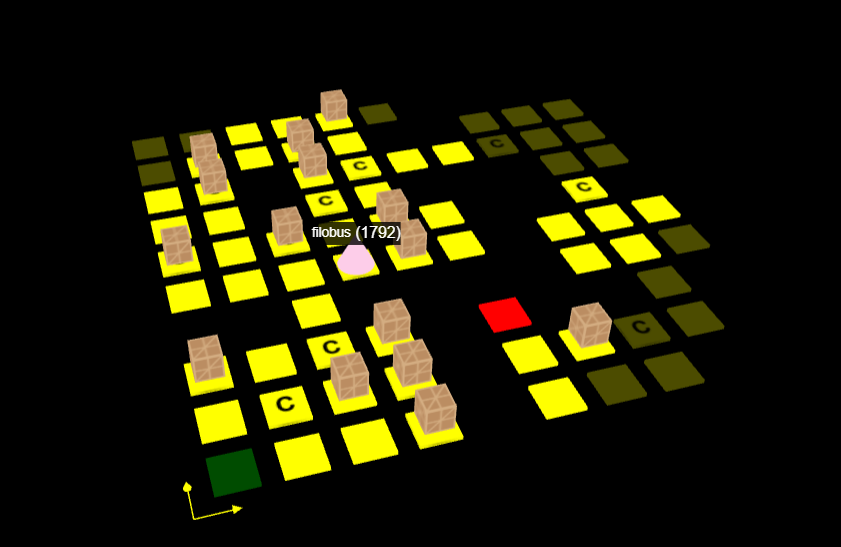
\includegraphics[width=0.72\linewidth]{crates_maze.png}
\caption{The \texttt{crates\_maze} map with Agent A (pink, \textit{filobus})
         mid-execution of a PDDL Sokoban plan.  Brown boxes labelled \textbf{C}
         are crates occupying yellow tiles; the red tile is the only delivery
         zone; the green tile (bottom-left) is the spawn zone.  The agent must
         push a subset of the 18 crates to open a path to the red delivery zone
         --- a configuration the A* planner cannot solve alone.}
\end{figure*}

\subsubsection*{Safety validation (\texttt{isPlanSafe})}
After the solver returns a plan, we validate it with a \emph{no-regression}
connectivity check: the plan is accepted only if the final crate configuration
leaves at least as many spawn zones connected to delivery zones (via crate-free
paths) as the initial configuration.  Formally, let $S_0$ be the set of spawn
zones connected to any delivery zone before the plan executes, and $S_f$ the
same set after simulating all pushes.  The plan is accepted if and only if
$|S_f| \geq |S_0|$.

This formulation correctly handles plans that \emph{temporarily} block
connectivity (e.g.\ moving a crate out of the way and restoring it) because the
final configuration is identical to the initial one, giving $|S_f| = |S_0|$.  An
absolute check ($|S_f| = |\text{all spawn zones}|$) would incorrectly reject
such reversible plans on maps where some spawn zones are not connected to
delivery zones in the baseline configuration.

\subsubsection*{Path cache}
To avoid redundant solver calls on periodic cycles (same start, goal, and crate
configuration), we maintain a static \texttt{Map} cache in
\texttt{PddlCratePlanner} keyed on
$\texttt{startX,startY} \to \texttt{goalX,goalY}:\texttt{crateHash}$, where
\texttt{crateHash} is the lexicographically sorted join of all crate positions.
Cache invalidation is implicit: if any crate moves, the hash changes and the
key misses.  Eviction uses FIFO at 30 entries.  Only plans that pass
\texttt{isPlanSafe} are stored.

\subsection{Complexity Discussion}

\begin{itemize}[noitemsep]
  \item \textbf{Navigation planner.}  With $T$ tiles the state space is $O(T)$
        (agent position), the branching factor is 4, and the problem is solvable
        in $O(T \log T)$ by A*; the PDDL formulation adds constant overhead from
        the solver.
  \item \textbf{Delivery planner.}  With $k$ parcel POIs and $z$ delivery zones
        the number of states is $O(2^k \cdot (k + z + 1))$ (carrying bitmask,
        agent position).  In practice $k \leq 8$, giving at most $256 \cdot 13
        \approx 3{,}000$ states — well within the solver's capacity.
  \item \textbf{Crate planner.}  This is the most complex instance.  The state
        space is $O(|T| \cdot \prod_i |Y_i|)$ where $|Y_i|$ is the number of
        yellow tiles reachable by crate $i$.  In the worst case (maze with 18
        crates, $|Y| \approx 10$ per crate) the theoretical space is enormous;
        in practice, the online solver finds plans in $\sim$3 s on
        \texttt{crates\_maze}.  The scoping limit (\texttt{MAX\_PDDL\_CRATES} = 20)
        caps the branching factor when many crates are present.
\end{itemize}

\subsection{Practical Trade-off}

Across the three planners, the only one whose cost-benefit trade-off proved
consistently positive was the Sokoban crate planner.  On crate-free maps it
is never invoked; on Sokoban maps it solves a problem A* simply cannot handle,
so the $\sim$3\,s solver latency is an unavoidable baseline rather than a
regression, and the path cache amortises it to near zero after the first cycle.

The navigation planner (\S\ref{sec:pddl}.1) and the task-level delivery planner
(\S\ref{sec:pddl}.2) degraded performance in most tested scenarios.  Both
introduce a round-trip to the online solver — typically 1--5\,s — for problems
that A* resolves locally in milliseconds.  That latency translates directly to
missed pickups and avoidable reward decay, making neither planner competitive
with the greedy baseline in the environments tested.  Both are therefore disabled
by default (\texttt{USE\_PDDL\_PLANNER} and \texttt{USE\_PDDL\_DELIVERY} default
to \texttt{false}) and kept as optional demonstrations of PDDL integration rather
than production-grade components.

% ============================================================
\section{Validation and Testing}
\label{sec:validation}
% ============================================================

Validation was carried out heuristically: both agents were deployed across
all available map configurations and exercised through a broad range of
scenarios, with the goal of stressing known design boundaries and
surfacing failure modes that do not appear in normal play.  Agent
behaviour was observed directly through console output and the live game
view; edge cases were reproduced manually until their root cause was
identified.

\subsection{Agent A: BDI on Standard and Crate Maps}

On maps without crates Agent A behaves robustly.  The utility function
($U = \hat{R}^2/d$) consistently favours nearby high-value parcels over
distant low-value ones, and the blacklist suppresses oscillation toward
temporarily unreachable targets.  Patrol fills idle cycles reliably,
directing the agent toward spawn zones not yet visited in the current round.

The most relevant failure mode on crate-free maps was the patrol
anti-livelock case: on small maps where every spawn zone falls within the
sensing radius simultaneously, the \texttt{notVisible} guard disqualifies
all patrol candidates, leaving the agent stuck in the deadlock-fallback
predicate indefinitely.  The fix — falling back to the \emph{nearest}
spawn regardless of visibility when no \texttt{notVisible} candidate
exists — was confirmed to resolve the issue on a minimal test map.

\texttt{crates\_one\_way} presented fewer problems than \texttt{crates\_maze}:
the agent navigated and delivered parcels with noticeably less interference
from crate-related path failures.

\texttt{crates\_maze} was the most demanding test, with the PDDL Sokoban
solver required frequently to unblock paths.  A structural weakness on this
map is the interaction between the online solver and the blacklist: if the
solver fails or times out, \texttt{CrateNavigate} returns \texttt{null}, the
delivery zone is blacklisted for \texttt{BAN\_DURATION\_MS}, and on
\texttt{crates\_maze} --- where the delivery zone is often the only reachable
target after a push --- the agent idles for the entire ban window with no
productive alternative.

\subsection{Agent B: LLM Agent under Mission Variety}

Agent B was tested with a wide range of natural-language missions to probe
both the LLM's plan generation and the executor's mechanical enforcement layer.

\textbf{Arithmetic coordinate missions} (e.g.\ \emph{``move to
x\,=\,4\,*\,2, y\,=\,(1\,+\,3)\,*\,3''}) were handled correctly in all
trials.  The LLM consistently identified the expression syntax and passed
the raw string to \texttt{navigate\_to}, which resolves it through
\texttt{safeEvalArithmetic} rather than evaluating it inline.

\textbf{Extreme-tile missions} (e.g.\ \emph{``drop a package in the
leftmost tile''}) succeeded reliably once the pre-computed map extremes
were injected into the context.  The replanning loop served as a useful
correction mechanism for LLM inference errors (e.g.\ targeting a
non-walkable tile), as long as the failure is surfaced explicitly by the
executor via a descriptive error string.

\textbf{Batch delivery missions} (e.g.\ \emph{``deliver parcels in
stacks of exactly 3''}) were enforced correctly: the \texttt{put\_down}
gate blocked delivery until the carried count reached the batch
threshold, and opportunistic pickup was suppressed during transit to
prevent overshooting the target.  One recurring issue emerged when parcel
supply was low: waiting for enough spawns to fill the batch leaves the
agent idle, which the LLM sometimes misread as a plan failure,
triggering an unnecessary replan that reset the carry count to zero.

\textbf{Forbidden-tile missions} worked reliably.  The A* congestion-map
penalty of 100\,000 routes the agent around the designated tile in all
tested configurations, including cases where the tile lies on the natural
shortest path.  The only notable behaviour was a significantly longer
detour when the forbidden tile was the sole stepping-stone between two
map areas, which introduced extra decay that the LLM had not budgeted for
in its plan.

The most consistent weakness of Agent B is \textbf{plan incompleteness}:
the model occasionally returned a valid JSON plan that omitted a necessary
pickup or intermediate navigation step, requiring a replan.  This was most
frequent on missions involving multiple parcels across different map areas,
where the LLM's greedy nearest-first tendency conflicts with missions that
require a specific delivery order or location.

A second weakness is \textbf{context drift} on long sessions: the 8-entry
rolling memory eventually stops containing early outcomes, and the LLM can
revisit strategies it already found ineffective.  This manifested during
extended relay tests, where the agent occasionally reverted to direct
delivery instead of dropping parcels for the BDI partner before the relay
constraint in the current prompt corrected its course.

\subsection{Multi-Agent Coordination}

The closest-commits heuristic was effective whenever the two agents were
spatially separated: each targeted a different parcel with no message
overhead, and combined throughput was visibly higher than either agent
alone.  Occasional collisions (both agents committing to the same
parcel) were self-correcting, since the slower agent simply moves on to
the next candidate in \texttt{optionsGeneration}.

The freeze/release primitive was tested with a mission of the form
\emph{``stop Agent A and deliver all carried parcels yourself''}: Agent A
halted within one sensing tick and Agent B completed the delivery without
closest-commits competition.

Relay mode functioned correctly when both agents were active at the same
time.  When Agent A joined mid-session it missed the initial
\texttt{[COORD] rules relay=1} broadcast, but the periodic re-broadcast
(every 2\,s) caused it to enter relay mode within two ticks, an
acceptable delay in practice.

The main fragility in the coordination layer is \textbf{handoff timing}:
if Agent A is mid-movement when a \texttt{[COORD] fetch} message arrives,
it may complete the current move before processing the command, picking up
the wrong parcel first.  In practice this causes a one-cycle delay before
the correct parcel is retrieved, but on maps with fast reward decay it
introduces a measurable score penalty.

% ============================================================
\section{Conclusions}
\label{sec:conclusions}
% ============================================================

We have designed and implemented a complete multi-agent system for Deliveroo.js
that integrates three complementary planning paradigms: reactive A* pathfinding,
deliberative BDI reasoning with utility-based option generation, and symbolic
PDDL planning at task, navigation, and Sokoban obstacle levels.

\subsubsection*{Key results}
Agent A demonstrates that a well-tuned utility function (squared reward over
distance) combined with intention stability and a blacklist mechanism provides
robust, high-throughput behaviour in the default single-agent setting.  The
graduated PDDL integration (navigation $\to$ delivery sequencing $\to$ crate
recovery) shows that external planners can be introduced at increasing levels of
complexity without disrupting the reactive baseline: each PDDL module is gated
by runtime flags and fails gracefully.  Agent B demonstrates that a
Plan-and-Execute LLM agent with hybrid startup achieves near-zero perceived
latency while still leveraging the model's natural-language reasoning for free-text
mission interpretation, with significantly fewer LLM calls per objective than
a per-step reasoning loop would require.

\subsubsection*{Limitations and future work}
\begin{itemize}[noitemsep]
  \item \textbf{PDDL optimality.}  The delivery planner uses STRIPS without
        \texttt{:action-costs}; the returned plan minimises the number of actions,
        not travel distance.  Switching to \texttt{:numeric-fluents} +
        \texttt{:metric minimize (total-cost)} with A*-computed edge costs would
        yield distance-optimal multi-parcel tours.
  \item \textbf{Path cache scope.}  The Sokoban path cache keys on the agent's
        start position; cycles where the agent approaches the goal from different
        tiles cause cache misses.  Keying only on (goal, crate configuration) and
        storing the cached plan's start as metadata would allow the executor to
        enter the cached path mid-sequence, improving hit rates significantly.
  \item \textbf{PDDL solver availability.}  The online solver at
        \texttt{solver.planning.domains} introduces a network dependency.  A
        local solver (e.g.\ Fast Downward) bundled with the agent would
        eliminate latency variability and offline failures.
  \item \textbf{LLM context drift.}  On very long sessions the rolling memory
        buffer (8 entries) may not suffice to prevent the LLM from repeating
        errors seen early in the session.  A structured episodic memory with
        semantic retrieval (e.g.\ a small vector index) would address this.
  \item \textbf{Coordination robustness.}  The \texttt{[COORD]} protocol is
        reliable only when both agents are connected simultaneously; a late-joining
        partner does not automatically receive the current constraint snapshot.
        Adding a periodic heartbeat re-broadcast of the full \texttt{rules}
        snapshot (already partially implemented) would solve this.
\end{itemize}

% ============================================================
\section*{References}
\addcontentsline{toc}{section}{References}
% ============================================================

\begin{thebibliography}{9}

\bibitem{rao1995}
  Rao, A.S.\ \& Georgeff, M.P.\ (1995).
  ``BDI agents: From theory to practice.''
  \textit{Proc.\ First International Conference on Multi-Agent Systems (ICMAS)},
  312--319.

\bibitem{mcdermott1998}
  McDermott, D.\ et al.\ (1998).
  ``PDDL --- The Planning Domain Definition Language.''
  Technical Report CVC TR-98-003/DCS TR-1165,
  Yale Center for Computational Vision and Control.

\bibitem{yao2023}
  Yao, S., Zhao, J., Yu, D., Du, N., Shafran, I., Narasimhan, K.,\ \& Cao, Y.\ (2023).
  ``ReAct: Synergizing Reasoning and Acting in Language Models.''
  \textit{International Conference on Learning Representations (ICLR 2023)}.
  \url{https://arxiv.org/abs/2210.03629}

\bibitem{litellm}
  Berri AI.\ (2023).
  LiteLLM: Unified API for 100+ LLM providers.
  \url{https://github.com/BerriAI/litellm}

\bibitem{planningdomains}
  Planning.Domains.
  \textit{Online PDDL Solver Service}.
  \url{https://solver.planning.domains}

\bibitem{deliveroojs}
  Autonomous Software Agents Course, University of Trento.
  \textit{Deliveroo.js --- Course Scaffold}, A.A.\ 2025--2026.
  \url{https://github.com/unitn-ASA/DeliverooJs}

\end{thebibliography}

\end{document}

